% Written by src/detection/final_figures.py; needs \usepackage{graphicx} and results/figures/ in \graphicspath.
\begin{figure*}[tb]
  \centering
  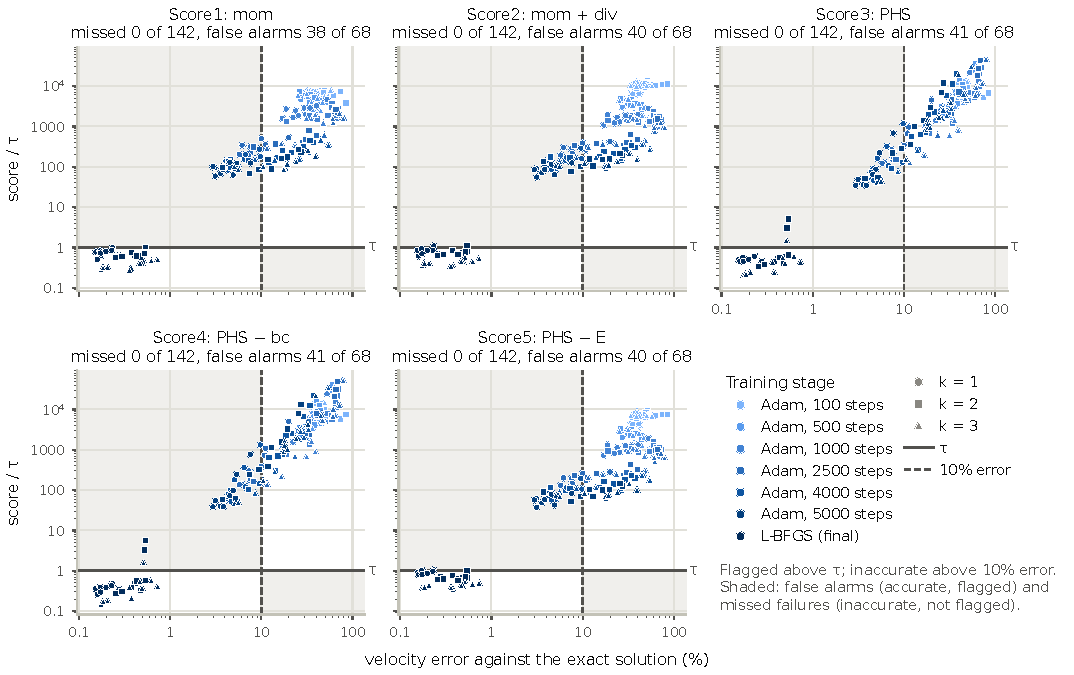
\includegraphics[width=\textwidth]{fig_natural_score_vs_error.pdf}
  \caption{The score of each of the 210 checkpoints of the 30 new runs (after 100, 500, 1000, 2500, 4000 and 5000 Adam steps, and the final model after L-BFGS) against its velocity error relative to the exact solution, on the $64\times64\times11$ test grid. Each score is divided by its frozen $\tau$, so the horizontal line at 1 is $\tau$ (flagged above it); dashed line: a model is inaccurate above 10\% error. Colour: the training stage, light to dark; marker: $k$. Shaded: where false alarms (accurate, flagged) and missed failures (inaccurate, not flagged) would lie. Every score flags all 142 inaccurate checkpoints. The false alarms are the 38 Adam checkpoints with errors from 2.96 to 10\%, which every score flags, and the false alarms on the 30 accurate final models (Score1 0, Score2 2, Score3 3, Score4 3 and Score5 2). No checkpoint has an error between 0.73\% (the least accurate final model, case\_58) and 2.96\% (the most accurate Adam checkpoint).}
  \label{fig:natural_score_vs_error}
\end{figure*}
